\section{Vendor instructions}
\subsection{Orders view}
By clicking on the \textit{Orders} button in the header, the seller reaches the orders page, where he can view all the orders placed by customers.
\newline
From this page the vendor can view for each order:
\begin {itemize}
\item the order code;
\item the status of the order;
\item the total and subtotal price;
\item the quantity of ordered items;
\item the checkout date;
\item the name of the customer who placed the order.
\end {itemize}
\begin{figure}[!ht]
    \caption{Orders page viewed from the vendor}
    \vspace{5px}
    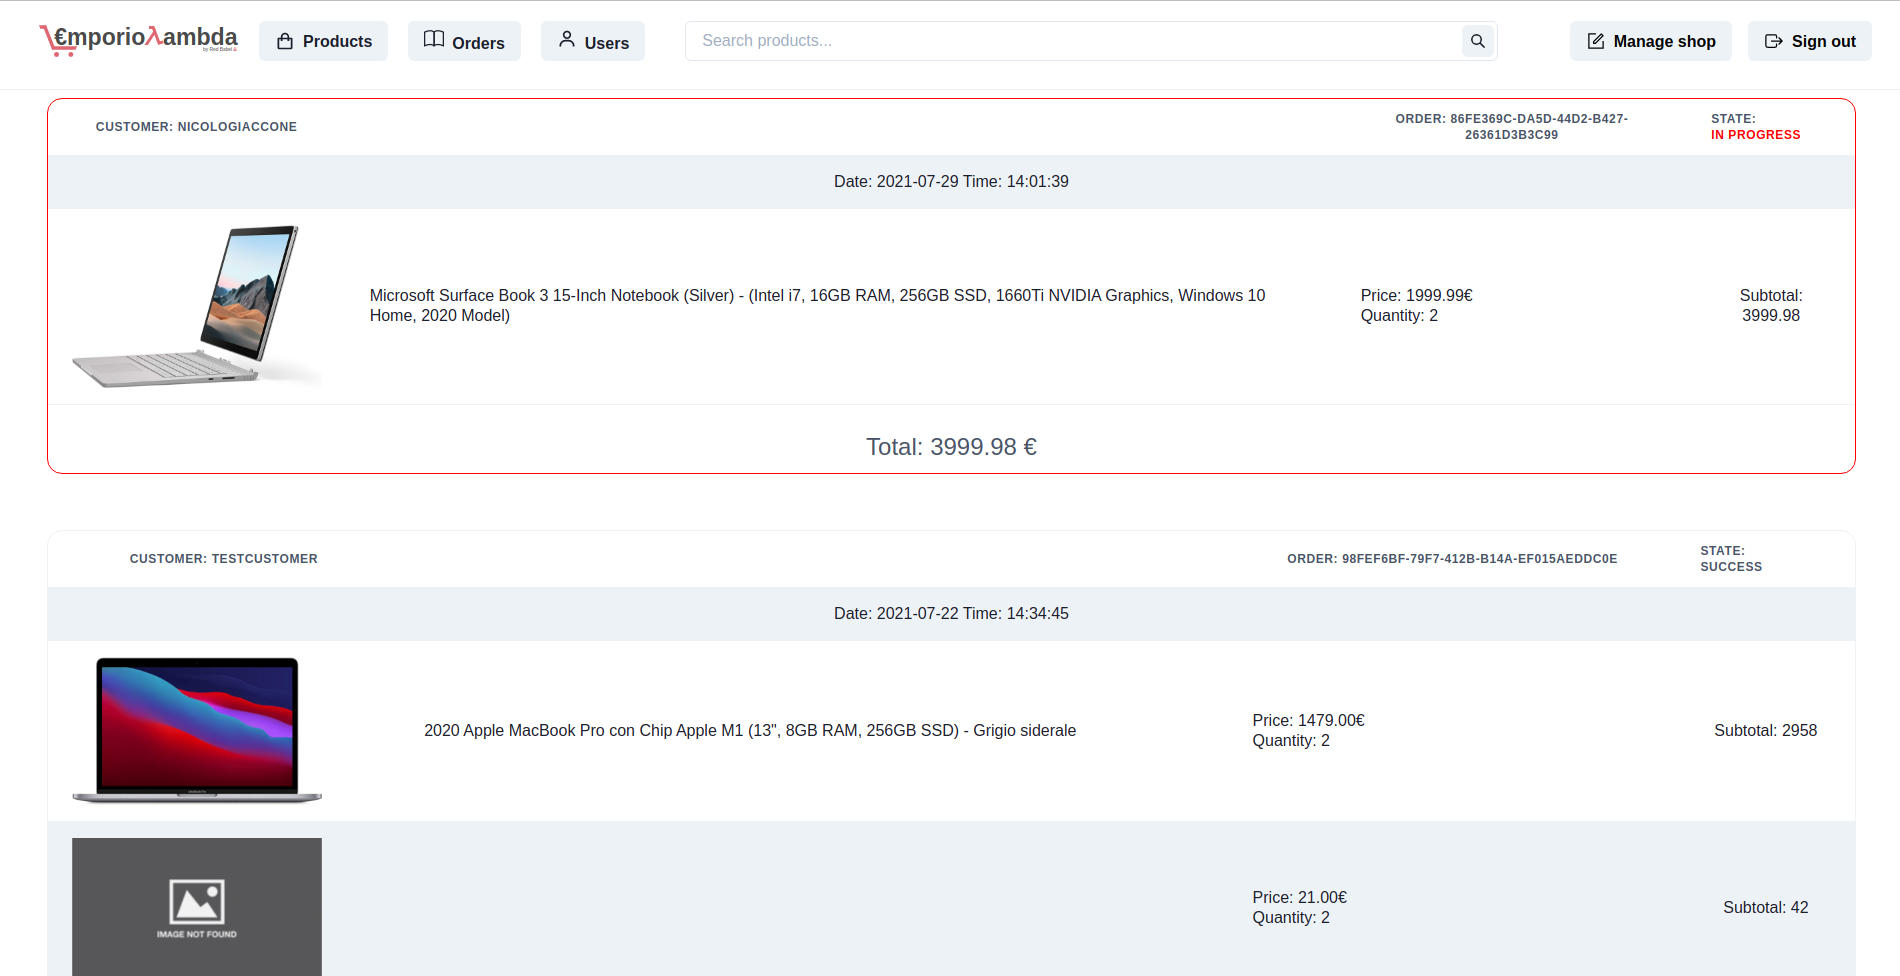
\includegraphics[scale=0.25]{../../../../Images/userManual/ordersVendor.png}
    \centering
\end{figure}
\pagebreak
\subsection{Shop management}
By clicking on the \textit{Manage shop} button in the header, the seller reaches the page to manage orders, where he can create a new product, create a new category or delete a category.
\subsubsection{Create new product}
\begin{figure}[!ht]
    \caption{Create new product page viewed from the vendor}
    \vspace{5px}
    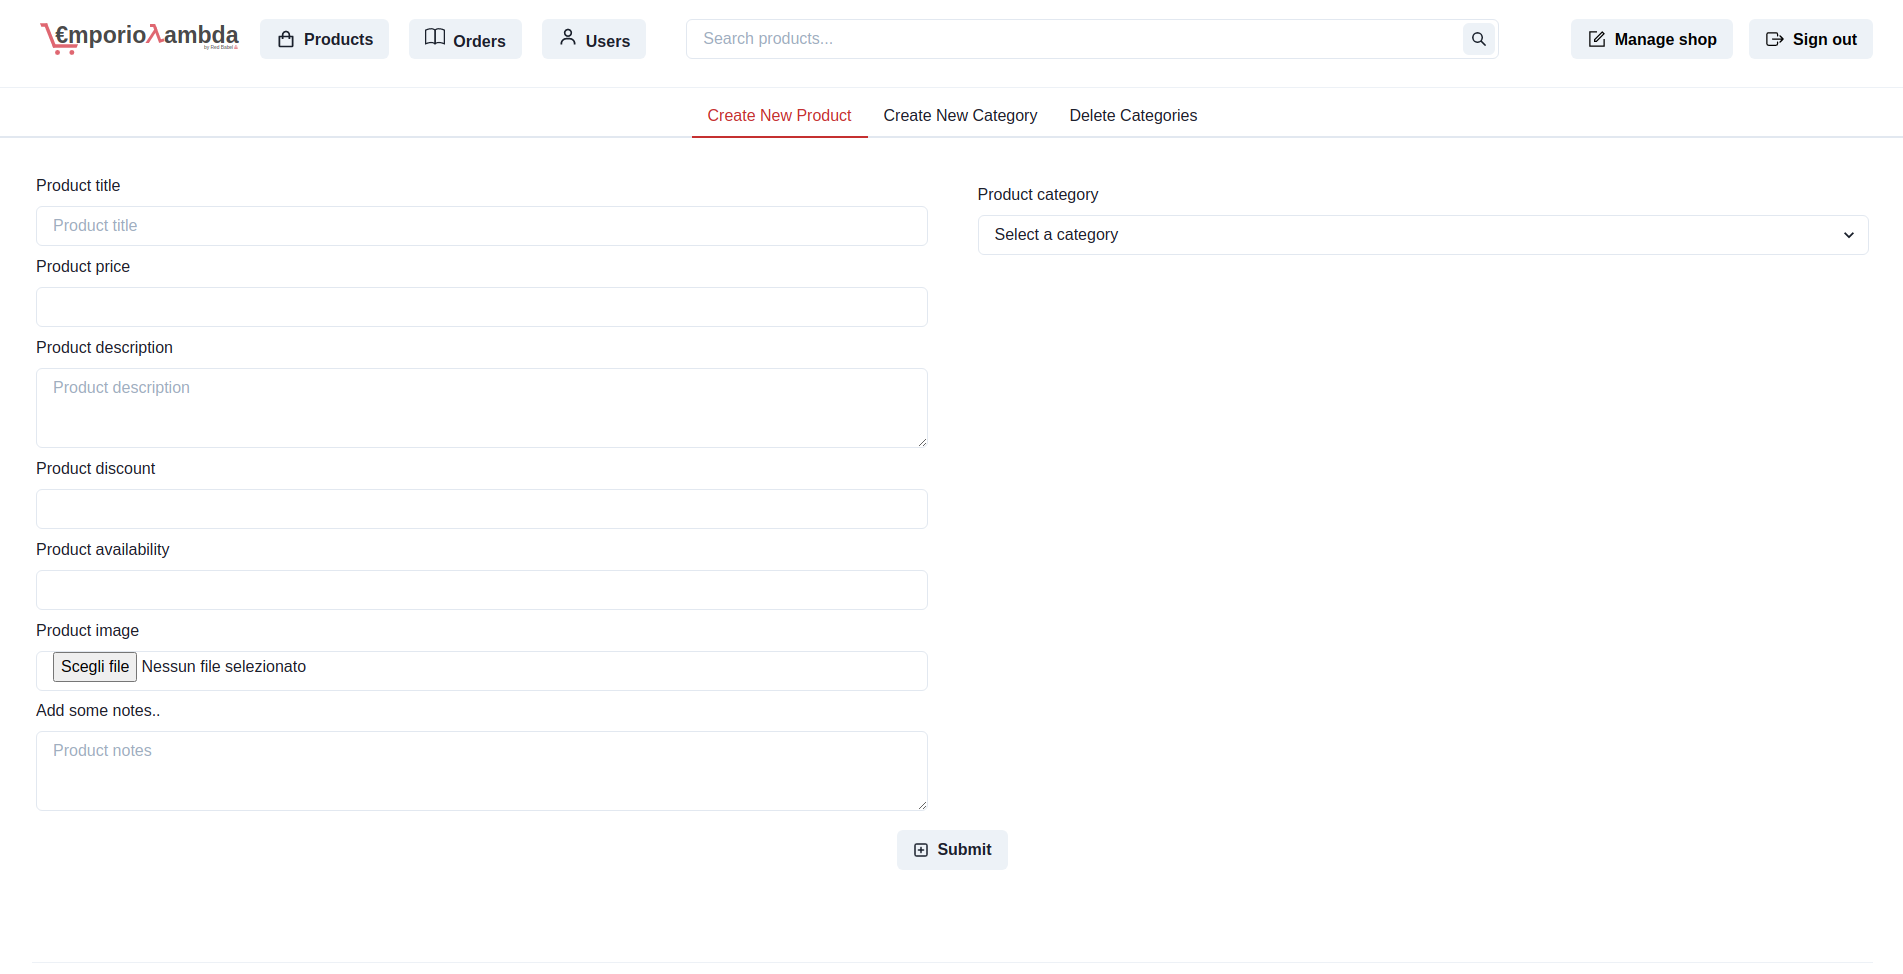
\includegraphics[scale=0.25]{../../../../Images/userManual/createNewProductVendor.png}
    \centering
\end{figure}
\pagebreak
\subsubsection{Create new category}
\begin{figure}[!ht]
    \caption{Create new category page viewed from the vendor}
    \vspace{5px}
    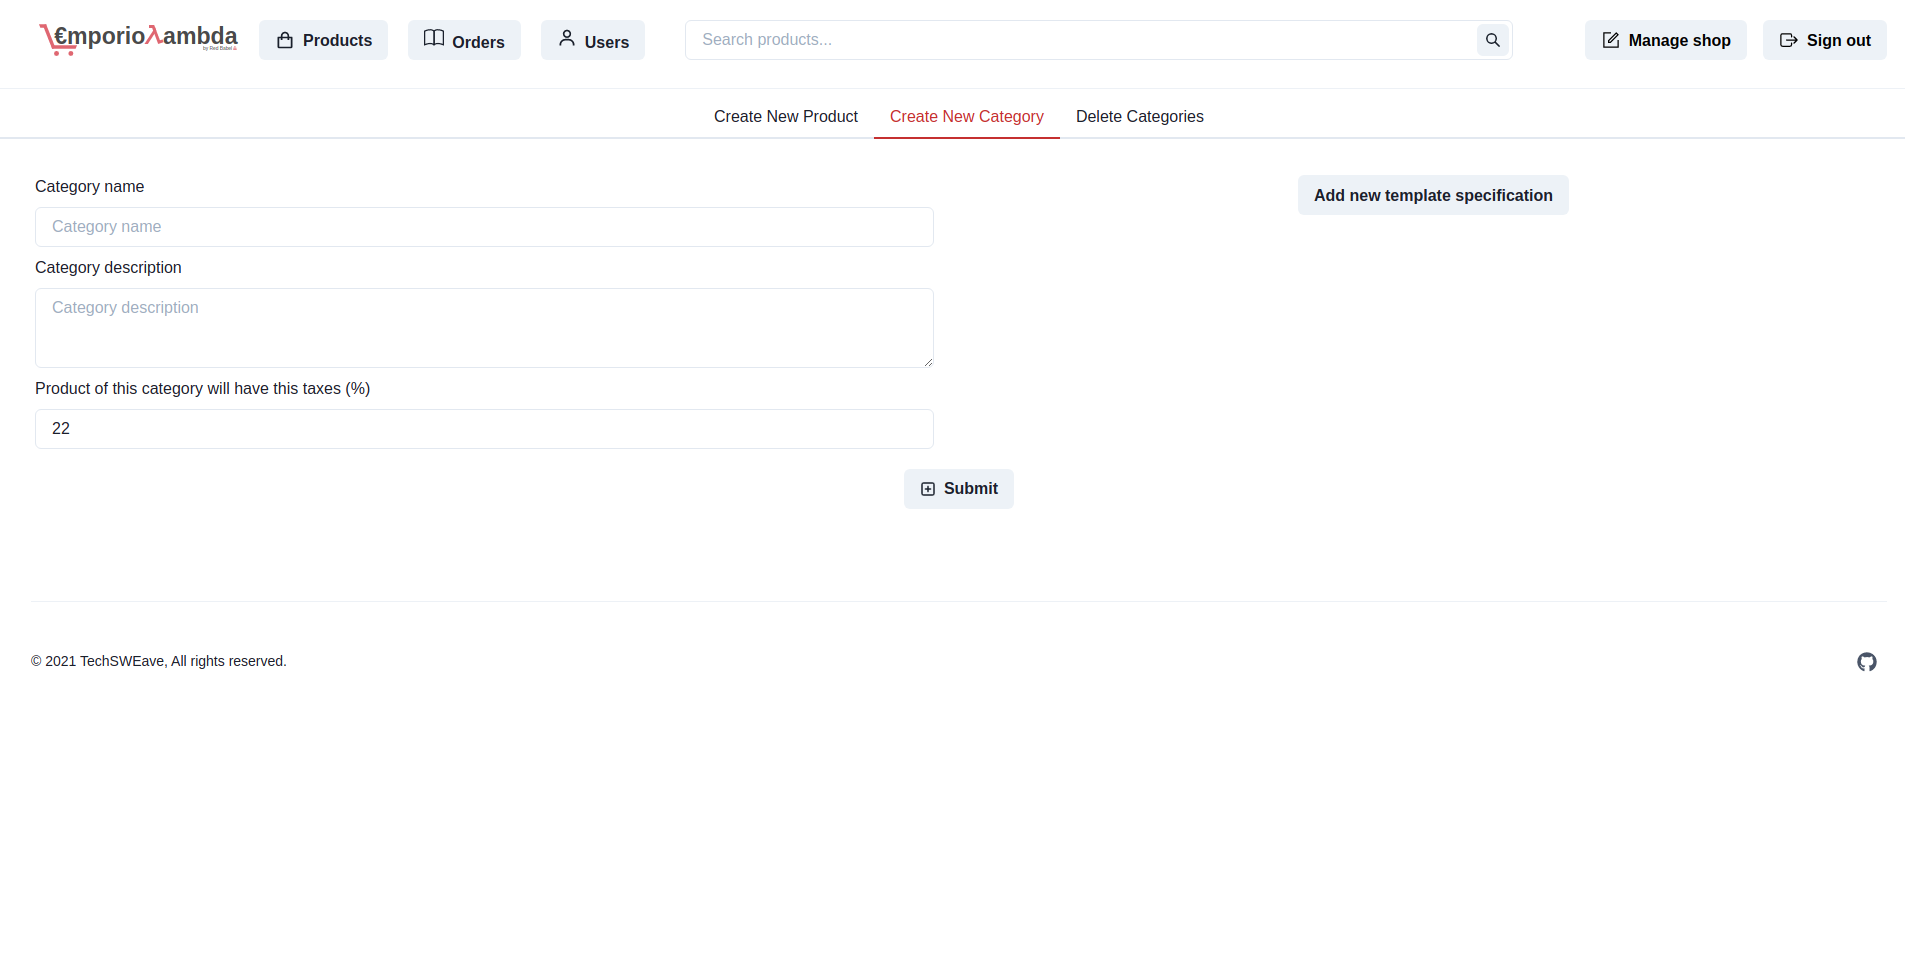
\includegraphics[scale=0.25]{../../../../Images/userManual/createNewCategoryVendor.png}
    \centering
\end{figure}
\pagebreak
\subsubsection{Delete categories}
\begin{figure}[!ht]
    \caption{Delete categories page viewed from the vendor}
    \vspace{5px}
    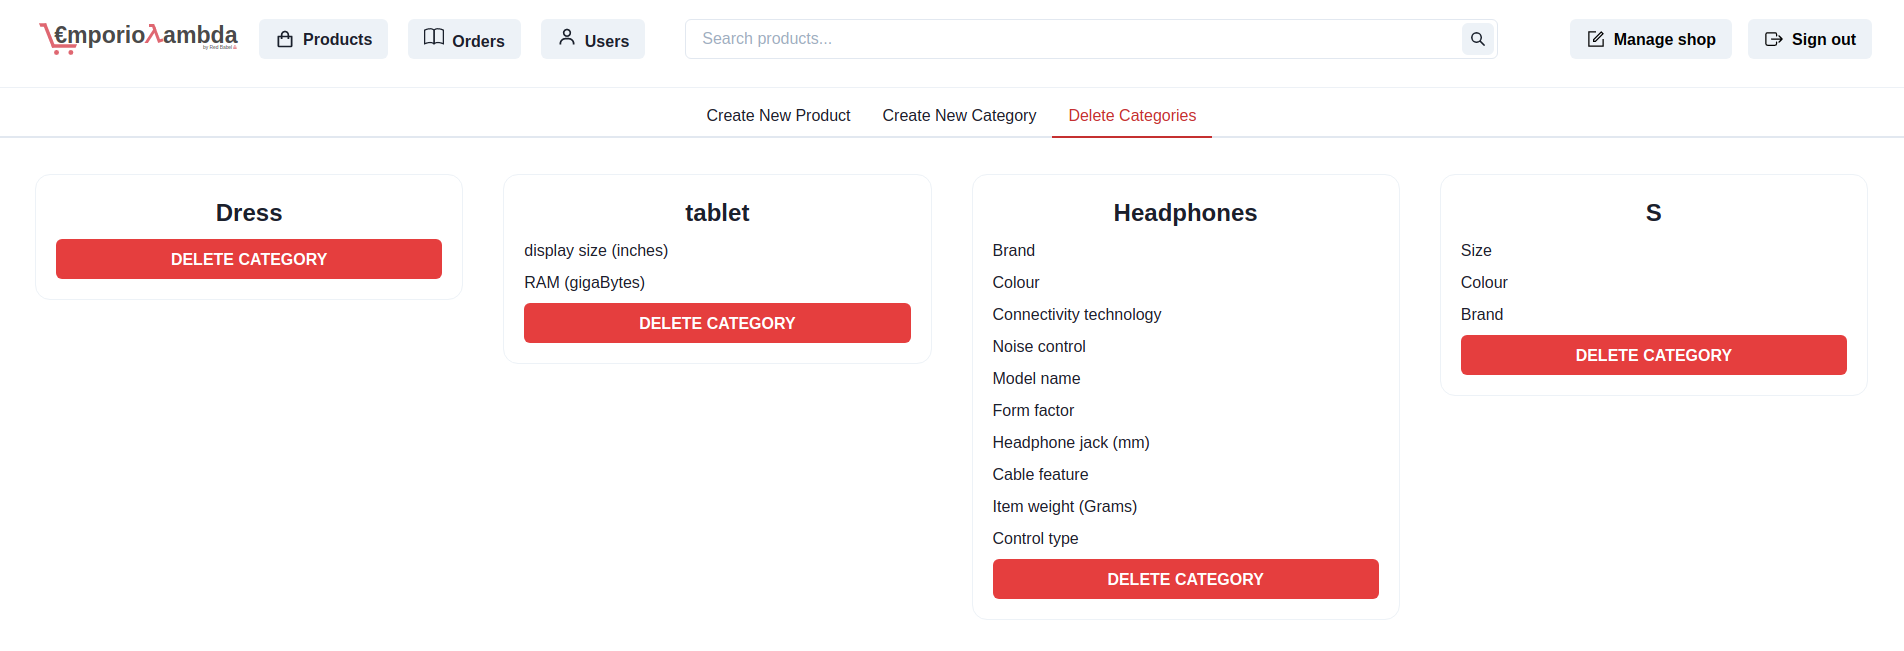
\includegraphics[scale=0.25]{../../../../Images/userManual/deleteCategoriesVendor.png}
    \centering
\end{figure}